
\section{Plotting in Python}

Python doesn't have any `native' data plotting tools but there are a
variety of packages that provide tools for visualizing data. The package
we're going to use is called `Matplotlib'. Matplotlib is one of the many
packages that is distributed with the Enthought Python distribution. If
you want to explore the full power of Matplotlib check out the example
gallery and the documentation at
\url{http://matplotlib.sourceforge.net/}.

\subsection{Basic plots using matplotib}

If you invoked the Ipython shell using the pylab option than most of the
basic matplotlib functions are already available to you. If not, import
them as so:

\begin{python}
>>> from pylab import *
>>> import numpy as np # go ahead and import numpy as well
\end{python}
\subsubsection{Loading data}

First let's load the yeast data set:

\begin{python}
>>> data = np.loadtxt('yeast-subnetwork-clean.txt',skiprows=1,usecols=range(1,16))
>>> data.shape   # check the dimensions of the resulting matrix
(173, 15)
\end{python}
The \lstinline!skiprows! argument tells the function how many rows in
the data file you want to skip. In this case we skipped only the first
row which gives the variable names. The \lstinline!usecols! arguments
specificies which columns from the data file to use. Here we skipped the
first (zeroth) column which had the names of the conditions. The usecols
\lstinline!loadtxt! works when there is no missing data. Use
\lstinline!numpy.genfromtxt! instead when there are missing values. For
a full tutorial on how to use the \lstinline!numpy.genfromtxt! function
see
\url{http://docs.scipy.org/doc/numpy/user/basics.io.genfromtxt.html}.

\subsubsection{Histograms in Matplotlib}

Matplotlib has a histogram drawing function. Here's how to use it:

\begin{python}
>>> hist? # in Ipython calls the help function
>>> h = hist(data[:,0]) # plot a histogram of the first variable (column) in our data set
>>> clf() # clear the plot window, don't need this if you closed the plot window
>>> h = hist(data[:,0], bins=20) # plot histogram w/20 bins
>>> h = hist(data[:,:2])  # histograms of the first two variables    
\end{python}
There's no built in density plot function, but we can create a function
that will do the necessary calculations for us to create our own density
plot. This uses a kernel density estimator function in the scipy library
(included with EPD). Put the following code in a file called
\lstinline!myplots.py! somewhere on your \lstinline!PYTHONPATH!:

\begin{python}
# myplots.py

import numpy as np
from scipy import stats

def density_trace(x):
    kde = stats.gaussian_kde(x)
    xmin,xmax = min(x), max(x)
    xspan = xmax - xmin
    xpts = np.arange(xmin, xmax, xspan/1000.)
    ypts = kde.evaluate(xpts) # evalude the estimate at the xpts
    return xpts,ypts
\end{python}
You can then use the \lstinline!density_trace! function as follows:

\begin{python}
>>> import myplots
>>> h = hist(data[:,0], normed=True) # use normed=True so histogram 
                           # is normalized to form a prob. density
>>> x,y = myplots.density_trace(data[:,0])
>>> plot(x,y, 'red')    
\end{python}
\subsubsection{Boxplots in Matplotlib}

Box-and-whisker plots are straightforward in Matplotlib:

\begin{python}
>>> b = boxplot(data[:,0])
>>> clf()
>>> b = boxplot(data[:,:5]) # boxplots of first 5 variables
\end{python}
The \lstinline!boxplot! function has quite a few facilities for
customizing your boxplots. For example, here's how we can create a
notched box-plot using 1000 bootstrap replicates (we'll discuss the
bootstrap in more detail in a later lecture) to calculate confidence
intervals for the median.

\begin{python}
>>> boxplot(data[:,0], notch=1, bootstrap=True)    
\end{python}
See the Matplotib docs for more info.

\subsubsection{Scatter Plots in Matplotlib}

Scatter plots are also easy to create:

\begin{python}
>>> s = scatter(data[:,0], data[:,1])    
\end{python}
\subsection{3D Plots}

Recent version of Matplotlib include facilities for creating 3D plots.
Here's an example of a 3D scatter plot:

\begin{python}
>>> from mpl_toolkits.mplot3d import Axes3D
>>> fig = figure()
>>> ax = fig.add_subplot(111, projection = '3d')
>>> ax.scatter(data[:,0],data[:,1],data[:,2])
<mpl_toolkits.mplot3d.art3d.Patch3DCollection object at 0x1a0bbd70>
>>> ax.set_xlabel('Gene 1')
<matplotlib.text.Text object at 0x1a0ae7d0>
>>> ax.set_ylabel('Gene 2')
<matplotlib.text.Text object at 0x1a0bb2b0>
>>> ax.set_zlabel('Gene 3')
<matplotlib.text.Text object at 0x1a0bbcd0>
>>> show()
\end{python}
Retyping all those commands is tedious and error prone so let's turn it
into a function. Add the following code to \lstinline!myplots.py!:

\begin{python}
from matplotlib import pyplot
from mpl_toolkits.mplot3d import Axes3D

def scatter3d(x,y,z, labels=None):
    fig = pyplot.figure()
    ax = fig.add_subplot(111, projection='3d')
    ax.scatter(x,y,z)

    if labels is not None:
        try:
            ax.set_xlabel(labels[0])
            ax.set_ylabel(labels[1])
            ax.set_zlabel(labels[2])
        except IndexError:
            print "You specificied less than 3 labels."
    return fig
\end{python}
Now reload myplots and call the scatter3d function as so:

\begin{python}
>>> reload(myplots)
>>> myplots.scatter3d(data[:,0], data[:,1], data[:,2])
>>> myplots.scatter3d(data[:,0], data[:,1], data[:,2], lab)
>>> myplots.scatter3d(data[:,0], data[:,1], data[:,2],labels=('X','Y','Z'))
\end{python}
\section{Plotting Geographic Data using Basemap}

There are a number of toolkits available for Matplotlib that extend the
functionality of the package. The mplot3d is one of those toolkits which
has now been incorporated into the standard distribution. Basemap is
another toolkit that provides the ability to plot 2D data on maps. The
Basemap toolkit supports a variety of mapping projections and coordinate
transformations and has the ability to plot things likes water bodies
and political boundaries.

The EPD edition of Python includes Basemap but in the interest of space
they have removed the high resolution maps that the normal Basemap
distribution includes. In order to use those maps you can download a
basemap binary (for Windows) or the source code (on OS X) from the
\href{http://sourceforge.net/projects/matplotlib/files/matplotlib-toolkits/basemap-1.0.1/}{here}.

On Windows just run the executable installer (make sure you get the
version that is appropriate to your EPD distribution; either 32-bit or
64-bit).

On OS X, once you have downloaded the source tarball
(\lstinline!basemap-1.0.1.tar.gz!), open up a bash shell, navigate to
the directory where you saved the tarball, and type:

\begin{python}[language=bash]
tar xvzf basemap-1.0.1.tar.gz
\end{python}
This will decompress and unarchive the source code into a directory
called \lstinline!basemap-1.0.1!. Navigate to the directory where the
mapping data is stored:

\begin{python}[language=bash]
cd basemap-1.0.1/lib/mpl_toolkits/basemap/data
\end{python}
And then copy all the \lstinline!.dat! files to your Python
installation:

\begin{python}[language=bash]
cp *.dat /Library/Frameworks/Python.framework/Versions/Current/lib/python2.7/site-packages/mpl_toolkits/basemap/data
\end{python}
\subsection{Using Basemap}

In our first basemap example we show how to plot the US lower 48 and we
add a red dot to represent the city of Durham, NC. Save this code as
\lstinline!mapex.py! and run it from the command line
(\lstinline!python mapex.py!).

\begin{codeblock}[python]
# Derived from: Tosi, Sandro. Plotting Geographical Data using Basemap
# url: http://www.packtpub.com/article/plotting-geographical-data-using-basemap

import numpy as np
from matplotlib import pyplot
from mpl_toolkits.basemap import Basemap

# Lambert Conformal map of USA lower 48 states
m = Basemap(llcrnrlon=-119, llcrnrlat=22, urcrnrlon=-64,
  urcrnrlat=49, projection='lcc', lat_1=33, lat_2=45,
  lon_0=-95, resolution='l', area_thresh=10000)

# draw the coastlines of continental area
m.drawcoastlines()
# draw country boundaries
m.drawcountries(linewidth=2)
# draw states boundaries (America only)
m.drawstates()

# fill the background (the oceans)
m.drawmapboundary(fill_color='aqua')
# fill the continental area and lakes
m.fillcontinents(color='coral',lake_color='aqua')

# draw pt. indicating durham/raleigh area
# Durham, latitude:  35deg 52min N, longitude:78deg 47min W
dlat, dlong = 35.86, -78.78 # west is minus

# this maps latitude and longitude to map coordinates
mcoordx, mcoordy = m(dlong,dlat)
pyplot.plot(mcoordx,mcoordy, 'ro') # draw red dot
pyplot.text(mcoordx+36000, mcoordy-18000, 'Durham')

# finally show the file
pyplot.show()    
\end{codeblock}
%
In our second example let's assume you've been studying the population
genetics of the beautiful and rare North Carolina Blue Snouter (mammals
of the order Rhinogradentia; see Stümpke 1967. The snouters: form and
life of the Rhinogrades). You've been sampling snouter populations from
across NC and you want to make a figure for a paper showing all your
sampling locations. Download the file \lstinline!nc-sites.txt! from the
course wiki, and place it in the same directory as the following module
(\lstinline!mapex2.py!).

\begin{codeblock}[python]
# mapex2.py

import numpy as np
from matplotlib import pyplot
from mpl_toolkits.basemap import Basemap

m = Basemap(llcrnrlon=-85, llcrnrlat=33, urcrnrlon=-75,
  urcrnrlat=37, projection='lcc', lat_0=35.774, lon_0=-78.634,
  resolution='l', area_thresh=10000)

m.drawcoastlines()
m.drawcountries(linewidth=2)
m.drawstates()
m.drawmapboundary(fill_color='aqua')
m.fillcontinents(color='coral',lake_color='aqua')

sites = np.loadtxt('nc-sites.txt')

for row in sites:
    lat, lon = row[0], row[1]
    x,y = m(lon, lat) # note how longitude (x-direction) comes first
    # use blue +'s to plot sites
    pyplot.plot(x,y, 'b+', markersize=8,markeredgewidth=2) 

pyplot.show()    
\end{codeblock}
%
The \lstinline!mapex2.py! code will produce a figure like the one below.

\begin{figure}[htbp]
\centering
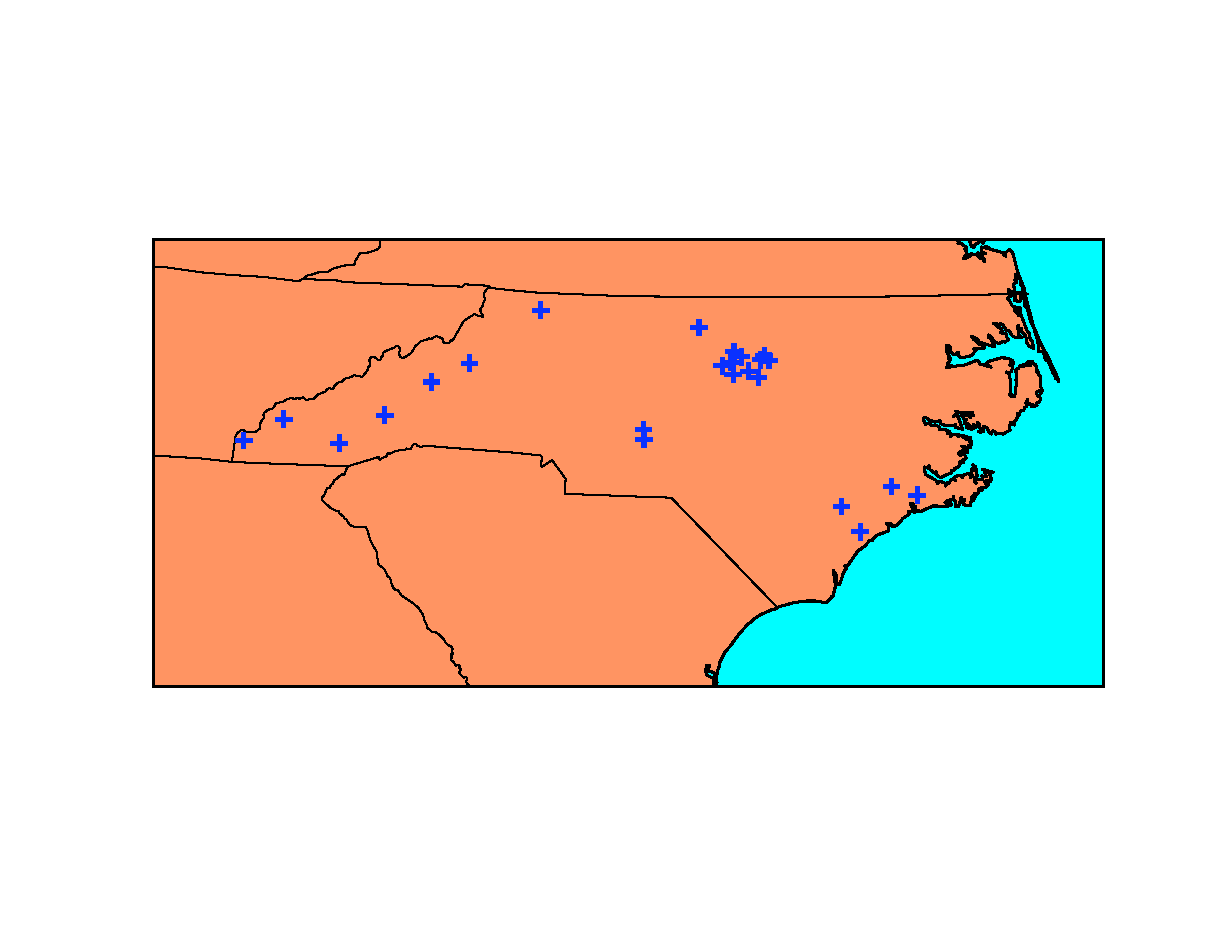
\includegraphics[width=0.6\columnwidth]{./figures/hands-on3/mapfig.pdf}
\caption{Output of the mapex2.py module}
\end{figure}
